\frame[plain]{\titlepage}
\frame{\frametitle{Outline}\tableofcontents}

\section{Problem - Nonlinear Real Arithmetic}
\subsection{Search Space of SMT(NRA)}

\begin{frame}
    \frametitle{Syntax of SMT(NRA)}
    
    polynomial: $p ::= x \mid c \mid p + p \mid p - p \mid p \times p$

    atoms: $a ::= b \mid p = 0 \mid p > 0 \mid p < 0$

    formula: $f ::= a \mid \neg f \mid f \wedge f \mid f \vee f $

    \vspace{0.4cm}

    SMT: Determine whether the formula is satisfied by some assignment (local search focuses), or prove unsat

    \vspace{0.4cm}

    Example:
    \\
    $x^2 + y^2 \le 1 \wedge x + y < 1 \wedge x + z > 0$
    \\
    assignment with $\left\{x \rightarrow 0, y \rightarrow 0, z \rightarrow 1\right\}$ satisfies all clauses.
\end{frame}

\begin{frame}{Fragment of Local Search (1)}
    \begin{algorithm}[H]
    \SetKwBlock{Begin}{}{}
    \SetAlgoLined
    \SetKwInOut{Input}{Input}
\SetKwInOut{Output}{Output}
\Input{A set of clauses $F$}
\Output{An assignment of variables that satisfy $F$, or failure}
Initialize assignment to variables\;
\While{$\top$}{
    \If{all clauses satisfied}{
        \Return{success with assignment\;}
    }
    \If{time or step limit reached}{
        \Return{failure\;}
    }
    Critical move procedure.
}
    \caption{Basic Fragment of Local Search\footfullcite{CaiLZ22}}
    \end{algorithm}
\end{frame}

\begin{frame}{Fragment of Local Search (2)}
    \begin{algorithm}[H]
    \SetKwBlock{Begin}{}{}
    \begin{minipage}{0.45\textwidth}
        \caption{First Part of the Algorithm}
        $\mathit{var,new\_value,score} \leftarrow$ best move according to make-break score\;
    \If{score $>$ 0}{
        Move $\mathit{var}$ to $\mathit{new\_value}$\;
    }
    \Else{
        Update clause weight\;
    }
    \end{minipage}
    \hfill
    \begin{minipage}{0.45\textwidth}
        \caption{Second Part of the Algorithm}
        \Repeat{3 times}{
            $\mathit{cls} \leftarrow$ random unsatisfied clause\;
            $\mathit{var,new\_value,score} \leftarrow$ critical move making $\mathit{cls}$ satisfied\;
            \If{score $\neq$ $-\infty$}{
                move $\mathit{var}$ to $\mathit{new\_value}$\;
            }
        }
        \If{no move performed}{
            Move some variables in unsatisfied clauses\;
        }
    \end{minipage}
    \end{algorithm}
\end{frame}
    

\begin{frame}
    \frametitle{Local Search for SAT and SMT}

    \begin{center}
        \begin{tabular}{|c|c|c|}
            \hline
            \diagbox{LS}{Problem}&SAT&SMT\\
            \hline
            Operation (Move)&Flip&Critical Move\\
            \hline
            Score Definition & \multicolumn{2}{c|}{Weighted unsat clauses}\\
            \hline
            Score Computation & Cached score& No Caching, time costly\\
            \hline 
            \end{tabular}
    \end{center}

    \textbf{What LS for SAT brings us: }\\
    Maintain scoring information after each iteration.\\
    \textbf{Difficulty:}\\
    Predetermine critical move shift value.\\
    \textbf{Our Solution:}\\
    Introduce Scoring Boundaries.
\end{frame}

\subsection{Current Existing Methods}

\section{Incremental Computation of Variable Scores}
\subsection{Scoring Boundary for Arithmetic Variable}

\begin{frame}{Make-break Intervals}
    \textbf{make-break intervals\footfullcite{abs-2303-06676}} \\
    Combination of (in)feasible intervals of arithmetic varaible $x$ with respect to all clauses.

    \begin{example}
        Current assignment: $\left\{ x\mapsto 1, y\mapsto 1, z\mapsto 1 \right\}$ \\
        Calculate infeasible set for each clause.
        \begin{itemize}
            \item $x^2+y^2\le 1$ (unsat): $(-\infty, 0) \cup (0, \infty)$.
            \item $x+y<1$ (unsat): $[0,\infty)$.
            \item $x+z>0$ (sat): $(-\infty,-1]$.
        \end{itemize}
        Combined information: $x$: $(-\infty,-1]\mapsto 0$, $(-1,0)\mapsto 1$, $[0,0]\mapsto 1$, $(0,\infty)\mapsto 0$.
    \end{example}
\end{frame}

\begin{frame}{Traditional Computation}
    \begin{algorithm}[H]
        \SetKwBlock{Begin}{}{}
        \SetAlgoLined
        \SetKwInOut{Input}{Input}
    \SetKwInOut{Output}{Output}
    \Input{unsat clauses $F$}
    \Output{Best critical move (variable, value)}
    \ForEach{variable $v$ in unsat clauses}{
        \ForEach{unsat clause $c$ with $v$}{        Compute interval-score info of $v$ in $c$.
        }
        Combine interval-score information. \\
        Update best var-value move.
    }
    \Return{best critical move}
    \end{algorithm}
    
    \vspace{0.4cm}
    \textbf{Repeated computation:}\\
    \begin{itemize}
        \item variable's (in)feasible set
        \item clause's sat staus
    \end{itemize}

\end{frame}

\begin{frame} 
    \frametitle{Boundary}
    \textbf{Definition.} A quadruple $\langle \mathit{val}, \mathit{is\_open}, \mathit{is\_make}, \mathit{cid}\rangle$, where $\mathit{val}$ is a real number, $\mathit{is\_open}$ and $\mathit{is\_make}$ are boolean values, and $\mathit{cid}$ is a clause identifier.
    \vspace{0.4cm}
    \begin{alertblock}{Meaning}
        \begin{itemize}
            \item $val:$ make-break value.
            \item $is\_open:$ active or not at $val$ point.
            \item $is\_make:$ make or break, increase or decrease score.
            \item $cid:$ causing clause.
        \end{itemize}
    \end{alertblock}

    \textbf{Sorting} First ordered by $val$, then by $is\_open$ ($\bot<\top$).
\end{frame}

\begin{frame}
    \frametitle{Boundary}
    Current assignment: $\left\{ x\mapsto 1, y\mapsto 1, z\mapsto 1 \right\}$ \\
    \begin{itemize}
        \item $x^2+y^2\le 1$: starting score 0, boundary set $\{(0,\bot,\top,1), (0,\top,\bot,1)\}$, indicating no change for large negative values, \emph{make} at boundary $[0,\cdots$, followed by \emph{break} at boundary $(0,\cdots$.
        \item $x+y<1$: starting score 3, boundary set $\{(0,\bot,\bot,2)\}$, indicating \emph{make} at large negative values, and \emph{break} at boundary $[0,\dots$.
        \item $x+z>0$: starting score $-2$, boundary set $\{(-1,\top,\top,3)\}$, indicating \emph{break} at large negative values, and \emph{make} at boundary $(-1,\dots$.
    \end{itemize}
    sorted boundary set: $\{(-1,\top,\top,3),(0,\bot,\top,1),(0,\bot,\bot,2),(0,\top,\bot,1)\}$
\end{frame}

\subsection{Incremental Computation}

\begin{frame}{Boundary Example}
    boundary set: $\{(-1,\top,\top,3),(0,\bot,\top,1),(0,\bot,\bot,2),(0,\top,\bot,1)\}$
    \vspace{0.2cm}
    \begin{center}
        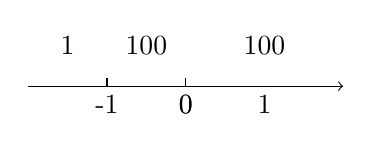
\begin{tikzpicture}
            \draw[->] (-2,0)--(2,0);
            \foreach \x in {1,2}
            {
                \draw[xshift=\x cm] (-2,0) -- (-2,0.1);
            };  
            \node[below] at (0,0){0};
            \foreach \x in {-1,0,1} {
                \node[below] at(\x,0){\x};
            }
            % starting score
            \node[below] at (-1.5,0.75){1};
            \node[below] at (-0.5,0.75){100};
            \node[below] at (1,0.75){100};
        \end{tikzpicture}
    \end{center}

    \textbf{Starting score:} Score when $x$ moves to -$\infty$. \\
    \textbf{Maintain and Change:} We maintain the boundary info for all arithmetic varaibles, unless the neighbour does a critical move.
\end{frame}

\begin{frame}{Algorithm for computing boundary}
    \begin{algorithm}[H]
        \SetKwBlock{Begin}{}{}
        \SetAlgoLined
        \SetKwInOut{Input}{Input}
    \SetKwInOut{Output}{Output}
    \Input{Variable $v$ that is modified}
    \Output{Make-break score for all variables}
    $S \leftarrow \{\}$ \tcp*{set of updated variables}
    \For{clause $\mathit{cls}$ that contains $v$}{
        \For{variable $v'$ appearing in $\mathit{cls}$}{
            add $v'$ to $S$\;
            recompute starting score and boundary of $v'$ with respect to $\mathit{cls}$\;
        }
    }
    \For{variable $v'$ in S}{
        recompute best critical move and score in terms of boundary information\;
    }
    \end{algorithm}
\end{frame}

\section{Temporary Relaxation of Equality (Non-Strick) Constraints}

\subsection{Difficulty in Local Search}

\begin{frame}{Previous Algorithm and Difficulty}
    \textbf{Number complexation in Local Search}


    When a variable chooses a complex value, the iteration is much slower, but sometimes we have to ...\\
    Reference\footfullcite{abs-2303-06676}  ignores equalities constraints due to its accurate value complexation.\\
    We introduce Relaxation into strick equality constraints, resulting in temporary interval candidate (rather than a point). \\
\end{frame}

\begin{frame}{Algebraic Numbers Situation}
    \begin{definition}[Complexity of values]
        We define a preorder $\prec_c$ on algebraic numbers as follows. $x\prec_c y$ if $x$ is rational and $y$ is irrational, or if both $x$ and $y$ are rational numbers, and the denominator of $x$ is less than that of $y$. We write $x \sim_c y$ if neither $x\prec_c y$ nor $y\prec_c x$.
        \end{definition}

    Algebraic (irrational) numbers have the largest complexity.
\end{frame}
\subsection{Relaxation Method}
\begin{frame}{Relaxation}
    \begin{Example}
        Given assignment $\left\{x\mapsto 1, y\mapsto 1\right\}$
        \begin{minipage}{0.45\textwidth}
            \centering
            $z^2 = x^2 + y^3$
        \end{minipage}
        % \hfill
        \begin{minipage}{0.45\textwidth}
            \centering
            $z^3 \ge 5 x^2 + y \vee z^3 \le 3x + 3y$
        \end{minipage}
        \end{Example}
        \vspace{0.6cm}
        Both situations force $z$ to an irrational number.

    \begin{alertblock}{Relaxation}
    \begin{itemize}
        \item If the constraint is of the form $p=0$, it is relaxed into the pair of inequalities $p<\epsilon_p$ and $p>-\epsilon_p$.

        \item If the constraint is of the form $p\ge 0$, it is relaxed into $p>-\epsilon_p$. Likewise, if the constraint is of the form $p\le 0$, it is relaxed into $p<\epsilon_p$.
    \end{itemize}
    \end{alertblock}
\end{frame}

\begin{frame}{Local Search with Relaxation}
    \scriptsize
    \begin{algorithm}[H]
\label{alg:relax}
\SetKwInOut{Input}{Input}
\SetKwInOut{Output}{Output}
\Input{A set of clauses $F$}
\Output{An assignment of variables that satisfy $F$, or failure}
Initialize assignment to variables\; 
\While{$\top$}{
    \If{all clauses satisfied}{
        $\mathit{success} \leftarrow$ find exact solution\;
        \If{success}{
            \Return{success with assignment};
        }
        \Else{
            Restore relaxed constraints to original form\;
            $\mathit{success} \leftarrow$ find exact solution by limited local search\;
            \If{success}{
                \Return{success with assignment};
            }
        }
    }
    \If{time or step limit reached}{
        \Return{failure}\;
    }
    Proceed traditional local search (slack).
}
    \end{algorithm}
\end{frame}

\section{Experiment}
\begin{frame}{Overall Result}
    \begin{table}[!t]
        \centering
        \small
        \begin{tabular}{c | c | c | c | c | c | c}
                    Category & \#inst & Z3 & cvc5 & Yices & ~Ours~ & ~Unique~ \\ \hline
                    20161105-Sturm-MBO & 120 & 0 & 0 & 0 & \textbf{88} & 88 \\
                    20161105-Sturm-MGC & 2 & \textbf{2} & 0 & 0 & 0 & 0 \\
                    20170501-Heizmann & 60 & 3 & 1 & 0 & \textbf{8} & 6 \\
                    20180501-Economics-Mulligan & 93 & \textbf{93} & 89 & 91 & 90 & 0 \\
                    2019-ezsmt & 61 & \textbf{54} & 51 & 52 & 19 & 0 \\
                    20200911-Pine & 237 & \textbf{235} & 201 & \textbf{235} & 224 & 0 \\
                    20211101-Geogebra & 112 & \textbf{109} & 91 & 99 & 101 & 0 \\
                    20220314-Uncu & 74 & 73 & 66 & \textbf{74} & 70 & 0 \\
                    LassoRanker & 351 & 155 & \textbf{304} & 122 & 272 & 13\\
                    UltimateAtomizer & 48 & \textbf{41} & 34 & 39 & 27 & 2 \\
                    hycomp & 492 & \textbf{311} & 216 & 227 & 304 & 11 \\
                    kissing & 42 & \textbf{33} & 17 & 10 & \textbf{33} & 1 \\
                    meti-tarski & 4391 & \textbf{4391} & 4345 & 4369 & 4351 & 0 \\
                    zankl & 133 & 70 & 61 & 58 & \textbf{100} & 27 \\ \hline
                    Total & 6216 & 5570 & 5476 & 5376 & \textbf{5687} & 148 
                \end{tabular}
        % \bottomrule
        % \multicolumn{4}{l}{\small $\bullet$ Solved by ours.}\\
        \end{table}
\end{frame}

\begin{frame}{Comparison}

\end{frame}

\begin{frame}[allowframebreaks]
    \frametitle{References}
\printbibliography
\end{frame}